\chapter{Introduction}
\label{sec:introduction}

The topic of this dissertation is an old idea in the
Internet---performance-enhancing proxies, or PEPs. But before I say more about
PEPs and all their triumphs and heartbreaks over the last few decades, I think
it's important to go through a brief history of the Internet. It will be
valuable to understand why certain aspects of the Internet were designed the
way they were so that we have the proper context for some of the challenges
they bring us today. Let's go back to the very beginning.

\section{Brief history of the Internet}

In the 1960s, the ARPANET was just a burgeoning research project sponsored by
the U.S. Department of Defense~\cite{hauben1997history}. The network consisted
of four stationary hosts,
including the Stanford Research Institute. ARPANET applied the new concept
of packet switching where data is broken down into smaller packets and
transmitted indepedently over wired links. Once the packets reach their
destination, they are reassembled into a message understandable by the
endpoint. Two computers communicated with each other for the first time in
1969~\cite{arpanet2019}. The first data transmitted over the network were the letters ``lo'' for
``login'', though the system crashed before the researchers could finish.

TCP/IP was introduced in the 1970s to provide a cleaner separation of
responsibilities between endpoints and in-network nodes as more and more
research institutions joined ARPANET~\cite{rfc675}. In this canonical model of
the Internet,
routers and other network components forward IP datagrams without regard to
their payloads, while TCP transport was end-to-end and implemented only in
hosts~\cite{saltzer1984endtoend,clark1988darpa}. The principles of packet
switching and TCP/IP are still present in how we use the network today.

In the 1980s, the early Internet was growing rapidly and the sheer amount of
traffic started to overwhelm the links. Network congestion caused packet loss,
which subsequently caused retransmissions and even more congestion, which led
to congestion collapse and a severe degradation in performance~\cite{rfc896}.
In response,
the first feedback control mechanisms for ``congestion control'' such as the
Van Jacobson algorithms for TCP/IP were invented~\cite{vjk}. Implemented at
hosts, these
``loss-based'' congestion control algorithms interpreted packet loss as
congestion to significantly decrease the congestion window.

The 1990s marked the beginning of the mainstream Internet, with the first
transatlantic links and the invention of the World Wide Web~\cite{www2025}. The
Internet was no longer just a research proposal, but a global commercial
project. Wi-Fi, which was
standardized in 1999, enabled people to move freely inside their homes and
workspaces~\cite{wifi2023}, while the iPhone and Android phones of the late
2000s along with the growth of cellular networks increased our mobility
elsewhere~\cite{smartphones2024}. Satellite
networks have long provided Internet access to remote and rural regions, and
are even more accessible today with low-Earth orbit satellites such as Starlink
in 2019~\cite{starlink2025}. Wireless networks and global connectivity really
expanded the reach of the Internet, but it also meant the network became more
lossy and high-delay than ever before.

Applications have also demanded more from the Internet over time, evolving from
basic services such as e-mail and web browsing to a continuous pursuit for
higher throughput and lower latency. There are high-bandwidth applications such
as streaming and content sharing (e.g., Netflix, YouTube, Instagram) and
interactive, low-latency applications such as video conferencing and live
streaming (e.g., Zoom, Twitch). Application goals often conflict---a service
like Netflix might prefer large buffers in the network to optimize for
throughput, while these same buffers introduce significant packet delays for
users of Zoom. When transport is end-to-end, a lossy, high-delay network
complicates how effectively hosts can coordinate and optimize performance for
the specific needs of their applications.

\subsubsection{Triumph: TCP performance-enhancing proxies.}

% How have the principles of TCP/IP and ``loss-based'' congestion control
% algorithms survived the test of time? The network still uses IP to route
% packets, and TCP and the loss-based CUBIC congestion control algorithm are
% still the networking defaults in the Linux kernel used by billions of devices
% today.

% The Internet today still uses TCP for transport, IP to route packets, and
% ``loss-based'' congestion control algorithms. Have these concepts survived the
% test of time for the networks and applications of the Internet today?

% In-network nodes use IP to route and forward
% packets, while TCP and the loss-based CUBIC congestion control algorithm still
% make up a significant portion of network traffic. Yet they don't quite exist
% in their original forms and.

% Although these TCP connections were originally end-to-end, as transport
% protocols were intended to be, PEPs interpose themselves in the path and split
% the connection into segments, each tuned to a different portion of the network.
% This break in end-to-end semantics allows PEPs to significantly improve
% performance in difficult environments, but comes at the cost of transparency,
% compatibility with encryption, and protocol evolution.


% Let's look at it in the context of QUIC, a relatively new transport protocol
% invented at Google in 2012 and standardized in 2021. If you have used Chrome,
% watched YouTube, or interacted with some other Google service, you have
% probably used QUIC. QUIC in some ways can be thought of as an alternative to
% TCP, offering ordering and reliability in the transport layer.

How do our resource-intensive applications deal with lossy, high-delay networks?
Let's examine the following scenario: Imagine you are riding the local commuter
rail. Your laptop is connected to the Wi-Fi on the train via a lossy,
low-latency wireless link to the router. The train's router then connects you
to the rest of the Internet via a more reliable, high-latency cellular path,
pinging nearby base stations that the train rides past. You upload a large file,
perhaps a paper submission to a conference. It's right before the deadline
and you find the network to be incredibly slow.

The router divides the network path into two very distinct path segments, but
from the perspective of the hosts' transport protocols on either end, there is
just \textit{one} lossy, high-delay network path. Because you need to upload
the entire file, when the wireless link drops a packet, you want to retransmit
the packet as soon as you find out about the loss. However, your laptop can
only detect the loss once it has received a signal from the web server on the
other end of the high-delay path, even though the loss occurred nearby.
Additionally, the ``loss-based'' congestion control on your laptop interprets
the signal as congestion, and decides to conservatively reduce the large
congestion window on the high-delay path by a significant amount. This slows
your connection down even more.

The solution to this problem in the 1990s when wireless networks first started
gaining popularity was performance-enhancing proxies, or PEPs~\cite{rfc3135}.
Now we can formally
define PEPs: PEPs are network middleboxes deployed to improve the
performance---most simply, throughput and latency---of the connections for
which they are on the path. These middleboxes were deployed widely at base
stations, satellite gateways, and even Wi-Fi routers. As of 2019, it was
estimated that 20--40\% of Internet paths still contained a
PEP~\cite{honda2011still, edeline2019bottomup}. Most
middleboxes provide in-network assistance to TCP, the dominant transport
protocol, and commonly as connection-splitting TCP PEPs~\cite
{kapoor2005achieving,caini2006pepsal,davern2011httpep,farkas2012splittcp,hayes2019mmwave}.
Other middleboxes
might perform header compression, ACK filtering and decimation, or other
caching and in-network retransmission functions to save bandwidth and improve
performance~\cite
{balakrishnan1995snoop,polese2017milliproxy,cronkite2016vcc,he2016acdc,mihaly2012mobilePEP}.

Your file upload could be much faster with a connection-splitting TCP PEP on the
train's router. These PEPs silently interpose themselves in the network path
without the knowledge of the endpoints, splitting
an end-to-end connection into multiple, independent TCP connections on either
side of the proxy. Once the connection is split, the proxy tunes congestion
control and other parameters for each, potentially very different, path
segment. Returning to the scenario on the train, the TCP transport protocol on
your laptop needs only to wait for a signal from the nearby router to detect
loss, as opposed to an end-to-end signal. The resulting congestion response is
also mild since the nearby congestion window is already small. The result is
earlier retransmissions and a significantly faster file upload.

\subsubsection{Heartbreak: Protocol ossification and secure transport protocols.}

However, even though there was a connection-splitting TCP PEP on the train, your
laptop was not using TCP but a different reliable transport protocol called
QUIC~\cite{rfc9000}. QUIC cannot benefit from PEPs made for TCP, and its
performance is the
same as an entirely end-to-end connection---slow. The irony in this situation
is that QUIC is a pretty new transport protocol announced in 2012, 38 years
newer than TCP and long after lossy, high-delay networks became the norm. It
was invented at Google, one of the world's largest software companies, and is
even in wide deployment with 8.4\% of websites supporting QUIC including major
traffic sources such as Cloudflare~\cite{zirngibl2021quicdeployment,w3techs,quiche}.
Yet its performance is so much worse, and
for reasons that were very intentional. How can this be explained?

Middleboxes cannot help QUIC because QUIC is what we call a ``secure'' transport
protocol. Even though transport was originally designed to be end-to-end, the
TCP transport headers in the payload of an IP datagram are unencrypted. This
reveals information such as the packet sequence number and acknowledgment
number to curious middleboxes. PEPs intercept the packets of a TCP handshake
and use this information to transparently split the connection on
initialization. In comparison, QUIC is completely encrypted on the wire. PEPs
are only able to forward these QUIC packets as opaque IP datagrams. Many recent
transport protocols in addition to QUIC now intentionally encrypt their
headers, rendering them unable to receive help from TCP PEPs and harming
performance~\cite{rfc8834webrtc,zoom,bittorrent,winstein2012mosh}.

If exposing transport headers to proxies can help performance, why are protocol
designers so deliberate about encrypting them? The answer lies in the sacrifice
that TCP made in hindsight to benefit from in-network assistance. To provide
the kind of help that they do, proxies make assumptions about the wire format
of the protocol and what each field is used for. They modify and block traffic
based on these fields. When protocol designers later repurpose these fields to
evolve the protocol or introduce new features, these assumptions break and the
``help'' can actually
harm~\cite{border2020quicsat-presentation,kuhn2021quic-over-sat,martin2022suitability,border2020evaluating,kosek2022quicpep}.
With PEPs being so widely deployed, backwards
compatibility is challenging to maintain and protocols have no choice but to
fix their functionality in place. This phenomenom is called protocol
ossification, where the wire format of the transport protocol has become
rigid and resistant to change over time~\cite{papastergiou2017deossifying, edeline2019bottomup}.

Protocol ossification has derailed the deployment of many otherwise promising
extensions to TCP. Despite making it as far as the IETF, ideas like
extended TCP options, Multipath TCP, ECN++, and tcpcrypt now lie in a graveyard
of unrealized proposals~\cite{mandalari2018ecnplusplus,honda2011still,raiciu2012multipathtcp,rfc8548}.
Even innocuously simple fields like the TCP sequence
number are not immune to ossification. For example, QUIC uses two sequence
number spaces, referring separately to packets and the bytes in the underlying
stream~\cite{rfc9000}. This is not possible with TCP. In one infamous debate,
exposing just a single bit in QUIC for passive RTT measurement triggered
widespread concern in the IETF about middlebox interference~\cite{quicbit2018}.
Due to stories like this, I would expect transport protocols to be secure by default
in the future.

An additional reason for encrypting the transport layer is privacy and security.
In the early days of the Internet, ARPANET was just a small network of trusted
research institutions. Privacy and security were not core design principles in
the invention of TCP/IP. Transport protocols these days prefer to limit the
exposure of non-essential information to network middleboxes using encryption.

\section{Overview}

This dissertation is about resolving the tension between performance and
ossification in PEPs for secure transport protocols. While existing work has
previously proposed co-designing PEPs with transport protocols~\cite{ford2008logjam,sherry2015blindbox, dogar2012tapa,iyengar2009flow},
I propose a new
approach to in-network assistance that leaves the original transport protocol
unmodified on the wire and free to evolve. In this approach, called \textbf
{Sidekick protocols}, proxies and endpoints send information \textit{about} the
packets of the underlying connection on an \textit{adjacent} connection.
Using a \textbf{Packrat proxy}, the adjacent connection can also generate
in-network retransmissions.
The information about the underlying connection is called a \textbf
{quACK}, which applies set reconciliation techniques to a novel setting to
efficiently refer to encrypted packets without plaintext sequence numbers.
I will show that \textcolor{black!50!blue}{\textbf{the Sidekick protocol
approach to in-network assistance for secure transport protocols achieves
performance benefits similar to those of traditional TCP PEPs without protocol
ossification}}.

The rest of this work will go as follows:
I will start \Cref{sec:quack} with quACKs, a tool for efficiently
referring to a set of randomly encrypted packets.
\Cref{sec:sidekick} will describe how proxies use the Sidekick protocol to send
quACKs over an adjacent connection, and how endpoints modify their behavior in
response to quACKs to emulate the performance benefits of traditional PEPs.
\Cref{sec:packrat} will describe how endpoints send quACKs to Packrat
proxies to receive in-network retransmissions, also achieving improved
performance for a variety of secure transport protocols.
Finally, \Cref{sec:splitting} will take a step back and analyze why recent
developments such as the ``model-based'' BBR congestion control algorithm and
the QUIC transport protocol may have cast doubts on the relevance of
connection-splitting, then offer a counterpoint.
\Cref{sec:conclusion} will describe future research directions and conclude.

\begin{figure}[t]
    \centering
    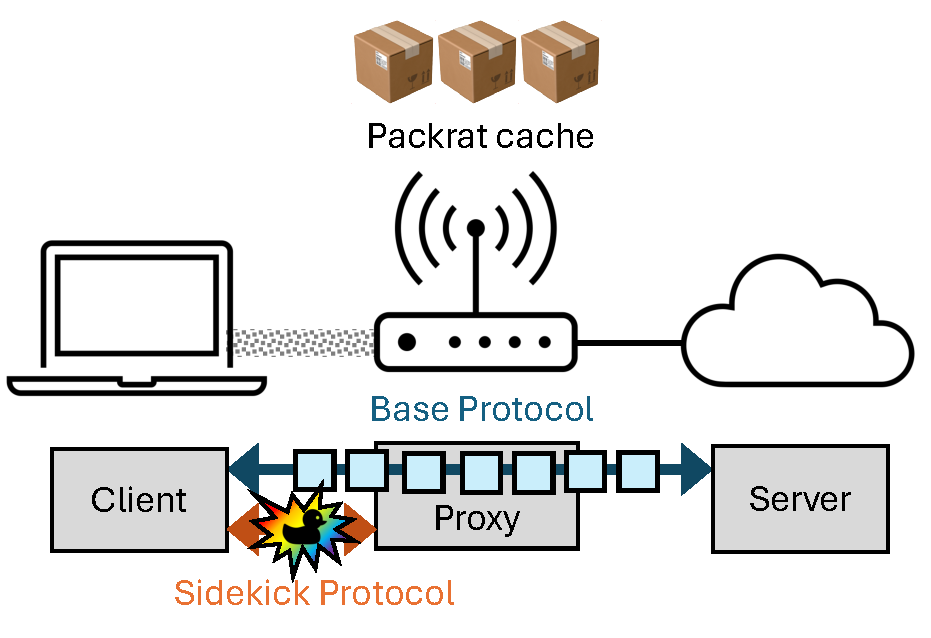
\includegraphics[width=0.7\linewidth]{slides/figures/overview.pdf}
    \caption{An overview of the Sidekick protocol approach to in-network
    assistance. In this diagram, the client is connected to the server
    via a lossy link to the proxy. The client and proxy speak the Sidekick
    protocol on an adjacent connection to the end-to-end connection between
    the client and server speaking the base protocol. QuACKs are exchanged
    over the Sidekick protocol, and the proxy also maintains a Packrat cache
    of packets for potential retransmission.}
    \label{fig:slides:overview}
\end{figure}


% \section{QuACKs: Referring to encrypted packets without sequence numbers}
% \label{sec:introduction:quacks}

% One of the main challenges of providing in-network assistance to secure
% transport protocols is how to usefully refer to packets when they do not have
% plaintext sequence numbers like TCP. In the first part of the dissertation,
% I will describe the quACK, a tool for efficiently referring to a set of
% randomly encrypted packets that a proxy or endpoint has received. The quACK
% applies set reconciliation techniques from more theoretical literature to
% communicate a small amount of information with efficient packet encoding and
% decoding times.

% \section{Sidekick: Secure in-network assistance for data senders}
% \label{sec:introduction:sidekick}

% Then, I will describe the Sidekick protocol for providing in-network assistance
% to data senders using secure transport protocols.
% The Sidekick approach is a fundamentally different type of architecture for
% in-network assistance. Rather than actively manipulating the connection on the
% wire by modifying and rewriting packets, the proxy simply observes the
% underlying connection, which we refer to as the base protocol. The proxy sends
% quACKs to the endpoint describing which packets it has received, and the
% endpoint makes path-aware decisions to enhance the performance of the
% connection while making the transport decisions end-to-end.

% \section{Packrat: Secure in-network retransmissions for data receivers}
% \label{sec:introduction:packrat}

% Next, I will present the Packrat protocol for helping secure transport protocols
% by sending in-network retransmissions to the endpoint. This scenario differs
% from that of the Sidekick protocol because the lossy path segment is near the
% data receiver instead of the data sender. This is challenging because the data
% sender dictates the terms of the data transfer, such as the sending rate and
% end-to-end retransmissions. However, there are also advantages in that the
% quACK sender is now co-located with the end-to-end ACK sender.

% \section{The future of connection-splitting with BBR and QUIC}
% \label{sec:introduction:heuristic}

% Taking a step back, recall that
% connection-splitting PEPs peaked in the late 1990s as a response to lossy,
% high-delay networks, and this was possible because TCP was unencrypted.
% Their utility today is complicated by post-TCP transport protocols such as QUIC
% that totally encrypt the transport layer on the wire. Sometimes what's old is
% new again, and sometimes what's old just needs to stay old.

% One of the core reasons QUIC was so slow in our train scenario was because of
% its congestion control algorithm's response to loss. In 2016, we had another
% advancement, also from Google, in the form of a new type of congestion control
% algorithm which is BBR. BBR was designed specifically for lossy, high-delay
% networks and is presumed to have much better performance. With options that are
% seemingly appealing for both ossification and performance, do recent
% developments such as BBR and QUIC truly make connection-splitting obsolete?

% We perform an emulation study of modern transport protocols and congestion
% control schemes both with and without connection-splitting PEPs, applying the
% \textit{split throughput heuristic}, and find that congestion control schemes do
% still benefit from connection-splitting today and the degree varies
% significantly by implementation. We present several takeaways regarding how to
% refer to end-to-end congestion control schemes and also hope this study
% motivates the need for protocol-agnostic forms of in-network assistance that
% emulate connection-splitting PEPs in the future.
